
% Experement data + calcs goes here %

\section{Ход работы}

\subsection{Зависимость B от тока через обмотку}

Данные представлены в таблице 1.

\begin{table}[h!] % Generated
    \begin{center}
    \begin{tabular}{|c|c|c|c|c|c|c|c|}
    \hline
    I, А   & 0,58 & 0,74 & 0,90 & 1,07 & 1,23 & 1,40 & 1,55 \\ \hline
    U, мТл & 608  & 750  & 880  & 972  & 1043 & 1088 & 1137 \\ \hline
    \end{tabular} \\ [0.2cm]
    \textit {Таблца 1: B (I).}
    \end{center}
\end{table}

\subsection{ВАХ для германия}

Данные представлены в таблице 2.

\begin{table}[h!] % Generated
    \begin{center}
    \begin{tabular}{|c|c|c|c|c|c|c|c|}
    \hline
    U, мкВ  & 327 & 673 & 1004 & 1178 & 1344 & 1501 & 1686 \\ \hline
    I, мA   & 0.2 & 0.4 & 0.6  & 0.7  & 0.8  & 0.9  & 1 \\ \hline
    \end{tabular} \\ [0.2cm]
    \textit {Таблца 2: ВАХ германия.}
    \end{center}
\end{table}

\noindentПолученная зависимость линейна. К-т наклона \mth{k\ruB{ВАХ} = 0,598 \pm 0,002 \,\frac{\texttt{А}}{\texttt{В}}} \\

\noindentПараметры образца: \mth{L_{35} = 3,0} мм; \mth{l = 1,7} мм; \mth{a = 1,3} мм. \\

\noindentТогда удельная проводимость образца: \mth{\sigma = \frac{IL_{35}}{U_{35}al} = 8,11 \pm 0,03 \,\frac{1}{\texttt{Ом} \cdot \texttt{см}}}

\subsection{Зависимость ЭДС Холла от B}

Для нескольких значений тока снял зависимоть ЭДС Холла от B.

\begin{table} [h!]
    \begin{center}
    \begin{tabular}{|c|c|c|c|} \hline
        B, мТл & Ux, мкВ & -Ux, мкВ & Uср, мкВ \\ \hline
        1137 & 515  & -434 & 474 \\ \hline
        1088 & 506  & -418 & 462 \\ \hline
        1043 & 483  & -397 & 440 \\ \hline
        972  & 458  & -370 & 415 \\ \hline
        880  & 416  & -335 & 376 \\ \hline
        750  & 367  & -287 & 327 \\ \hline
        608  & 300  & -224 & 262 \\ \hline
    \end{tabular} \\ [0.2cm]
    \textit{Таблца 3: ЭДС Холла от B для 1мА.}
    \end{center}
\end{table}

\newpage

\begin{table} [h!]
    \begin{center}
    \begin{tabular}{|c|c|c|c|} \hline
        B, мТл & Ux, мкВ & -Ux, мкВ & Uср, мкВ \\ \hline
        1137 & 267  & -222 & 245 \\ \hline
        1088 & 263  & -200 & 232 \\ \hline
        1043 & 247  & -192 & 221 \\ \hline
        972  & 235  & -182 & 209 \\ \hline
        880  & 215  & -163 & 190 \\ \hline
        750  & 188  & -137 & 163 \\ \hline
        608  & 157  & -106 & 132 \\ \hline
    \end{tabular} \\ [0.2cm]
    \textit{Таблца 4: ЭДС Холла от B для 0,5мА.}
    \end{center}
\end{table}

\begin{table} [h!]
    \begin{center}
    \begin{tabular}{|c|c|c|c|} \hline
        B, мТл & Ux, мкВ & -Ux, мкВ & Uср, мкВ \\ \hline
        1137 & 133  & -98  & 116 \\ \hline
        1088 & 131  & -95  & 113 \\ \hline
        1043 & 128  & -90  & 109 \\ \hline
        972  & 121  & -84  & 103 \\ \hline
        880  & 111  & -75  & 93  \\ \hline
        750  & 97   & -62  & 80  \\ \hline
        608  & 82   & -47  & 65  \\ \hline
    \end{tabular} \\ [0.2cm]
    \textit{Таблца 3: ЭДС Холла от B для 0,25мА.}
    \end{center}
\end{table}

На рисунке 3 представлены графики для этих данных:

\begin{figure}[h!]
    \center{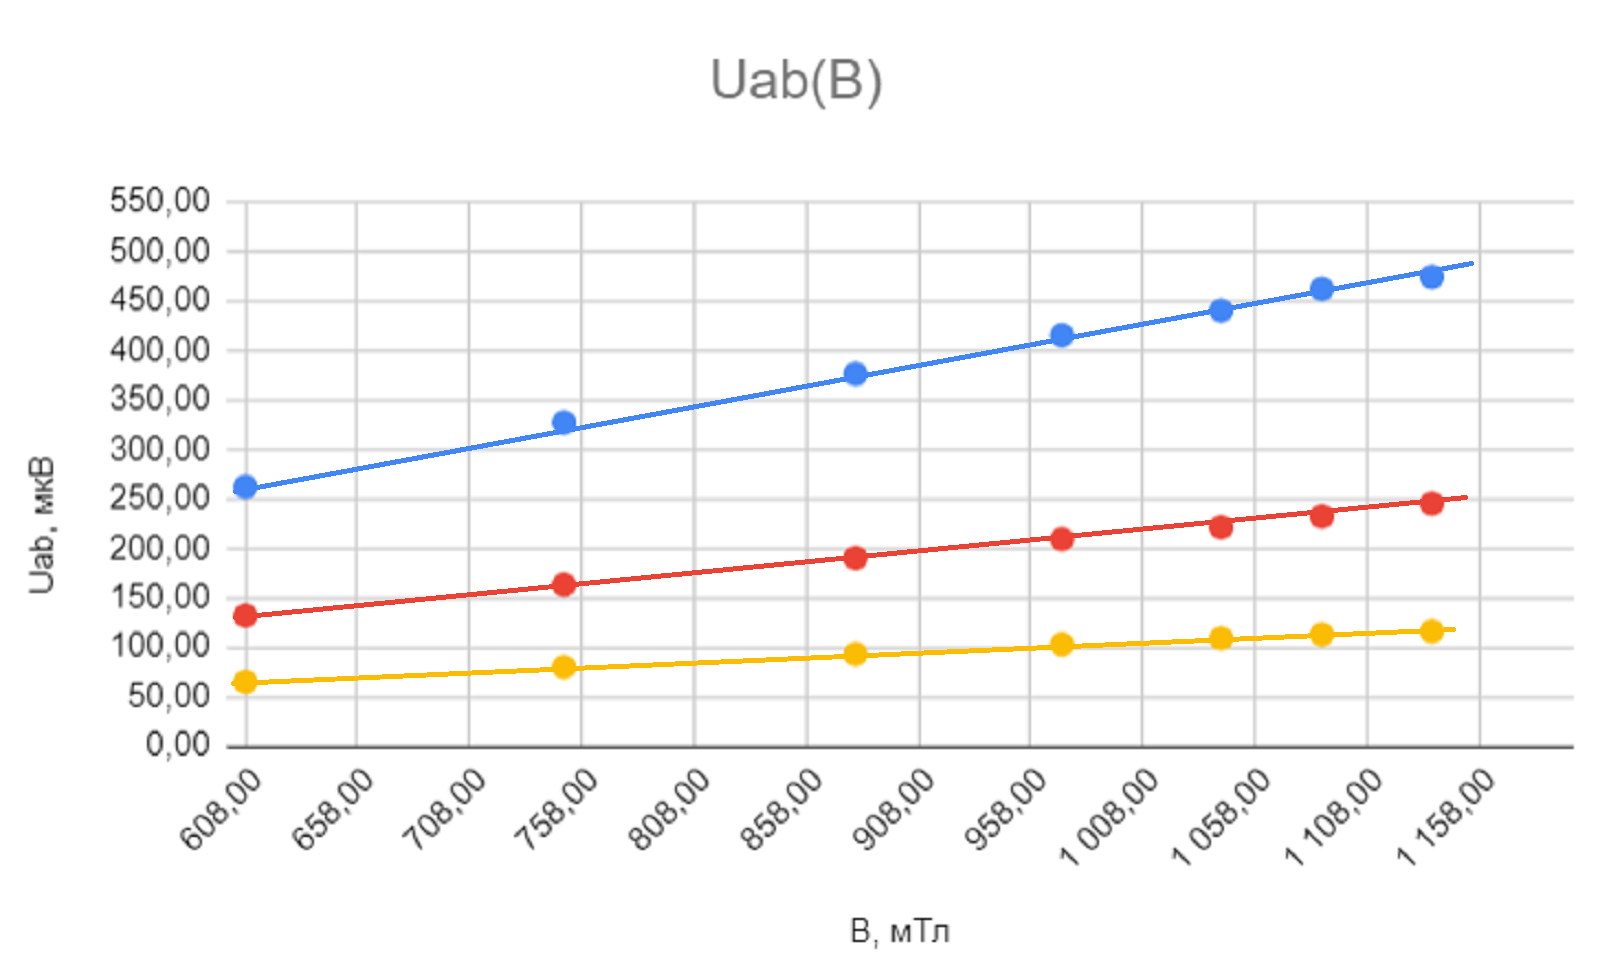
\includegraphics[width = 0.8\textwidth]{graph.png}}\\
    \textit{Рис. 3: Uab(B)}
\end{figure}

\newpage

\subsection{Рассчетные значения}

\noindentРассчетные значения для к-та Холла: \\

\noindent\mth{R_1 = \left( 54,9 \pm 0,3 \right) \cdot 10^{-5} \frac{\texttt{м}^3}{\texttt{Кл}}} \\

\noindent\mth{R_2 = \left( 55,6 \pm 0,3 \right) \cdot 10^{-5} \frac{\texttt{м}^3}{\texttt{Кл}}} \\

\noindent\mth{R_3 = \left( 55,1 \pm 0,3 \right) \cdot 10^{-5} \frac{\texttt{м}^3}{\texttt{Кл}}} \\

\noindentЗначения \mth{R_i} совпали с высокой точностью. \\

\noindentТакже рассчитал концентрацию носителей заряда в образце: \\
\mth{n = 11.2 \pm 0.1 \texttt{м}^{-1}} \\ 

\noindentИ подвижность носителей тока: \\
\mth{b = \left( 3,76 \pm 0,1 \right) \cdot 10^3 \frac{\texttt{см}^2}{\texttt{В}\cdot\texttt{с}}}

\section{Вывод}
В ходе данной лабараторной работы была снята зависимость ЭДС Холла от B. Данная зависимость оказалась линейной, что хорошо согласуется с теорией. Также по данной зависимости были рассчитаны к-т Холла, концентрация носителей заряда и подвижность носителей заряда. Значения для двух последних величин с высокой точностью совпали с табличными.